%% This Beamer template is based on the one found here: https://github.com/sanhacheong/stanford-beamer-presentation, and edited to be used for Stanford ARM Lab

\documentclass[10pt]{beamer}
%\mode<presentation>{}

\usepackage{media9}
\usepackage{amssymb,amsmath,amsthm,enumerate}
\usepackage{mathtools}
\usepackage[utf8]{inputenc}
\usepackage{array}
\usepackage[parfill]{parskip}
\usepackage[utf8]{vietnam}
\usepackage{graphicx,animate}
\usepackage{caption}
\usepackage{subcaption}
\usepackage{bm}
\usepackage{amsfonts,amscd}
\usepackage[]{units}
\usepackage{listings}
\usepackage{multicol}
\usepackage{multirow}
\usepackage{tcolorbox}
\usepackage{physics}
\usepackage{movie15}
% Enable colored hyperlinks
\hypersetup{colorlinks=true}

\usefonttheme{professionalfonts}

% The following three lines are for crossmarks & checkmarks
\usepackage{pifont}% http://ctan.org/pkg/pifont
\newcommand{\cmark}{\ding{51}}%
\newcommand{\xmark}{\ding{55}}%

% Numbered captions of tables, pictures, etc.
\setbeamertemplate{caption}[numbered]
\usepackage{media9} 
%\usepackage[superscript,biblabel]{cite}
%\usepackage{algorithmic}
%\usepackage{algorithm2e}
%\usepackage{algpseudocode}
\usepackage[linesnumbered,ruled,vlined]{algorithm2e}
%\usepackage{algorithm}
%\usepackage{algorithmic}
\usepackage{caption}
%\usepackage{xcolor}
\usepackage{array}
%\renewcommand{\thealgocf}{}

\usepackage[natbib,backend=biber,style=ieee, sorting=ynt]{biblatex}
\bibliography{ref.bib}

\usepackage[acronym]{glossaries}

\usepackage{graphicx}
\graphicspath{{./figures}}
\usepackage{hyperref}

\setbeamertemplate{theorems}[numbered]
\theoremstyle{remark}
\newtheorem{dl}{Định lý}
\newtheorem{md}{Mệnh đề}
\newtheorem{bd}{Bổ đề}
\newtheorem{dn}{Định nghĩa}
\newtheorem{hq}{Hệ quả}
%\theoremstyle{definition}

\numberwithin{algocf}{section}
\numberwithin{equation}{section}
\numberwithin{dl}{section}
\numberwithin{figure}{section}


%\newcommand{\empy}[1]{{\color{darkorange}\emph{#1}}}
%\newcommand{\empr}[1]{{\color{cardinalred}\emph{#1}}}
%\newcommand{\examplebox}[2]{
%\begin{tcolorbox}[colframe=darkcardinal,colback=boxgray,title=#1]
%#2
%\end{tcolorbox}}

%\usetheme{Stanford} 
%\input{./style_files_stanford/my_beamer_defs.sty}
\usetheme{Copenhagen}
\usecolortheme{seahorse}
%\logo{
\includegraphics[height=0.5in]{logos/HUS-name.jpg}}

\makeatletter
\let\@@magyar@captionfix\relax
\makeatother

\title[Mô hình khuếch tán xác suất]{Ước lượng ma trận hiệp phương sai tối ưu với trung bình không hoàn hảo trong mô hình khuếch tán xác suất}

\AtBeginSection[]
{
    \begin{frame}
        \frametitle{Nội dung}
        \tableofcontents[currentsection, subsectionstyle=show/show/hide]
    \end{frame}
}

\setbeamertemplate{page number in head/foot}[totalframenumber]
\setbeamertemplate{frametitle continuation}{}

\begin{document}
\author[Nguyễn Chí Thanh - 21007925]{
	\begin{tabular}{c} 
	\Large
	Nguyễn Chí Thanh \\
    \footnotesize \href{mailto:nguyenchithanh\_sdh21@hus.edu.vn}{nguyenchithanh\_sdh21@hus.edu.vn}
\end{tabular}
\vspace{-4ex}}

\institute{
	\vskip 5pt
	\begin{figure}
		\centering
		\begin{subfigure}[t]{0.5\textwidth}
			\centering
			
\includegraphics[height=0.75in]{logos/HUS-logo.jpg}
		\end{subfigure}%
		~ 
		\begin{subfigure}[t]{0.5\textwidth}
			\centering
			
\includegraphics[height=0.75in]{logos/MIM-logo.png}
		\end{subfigure}
	\end{figure}
	\vskip 5pt	
	Đại học Quốc Gia Hà Nội \\
	Trường đại học Khoa học tự nhiên\\
	Khoa Toán - Cơ - Tin học
	\vskip 3pt
}

%\begin{noheadline}
\begin{frame} \maketitle \end{frame}
%\end{noheadline}
    
\setbeamertemplate{itemize items}[default]
\setbeamertemplate{itemize subitem}[circle]

\begin{frame}{Nội dung}
    \tableofcontents[hidesubsections]
\end{frame}

\section{Tổng quan về mô hình khuếch tán xác suất}

\subsection{Tổng quan các mô hình sinh}

\begin{frame}
    \begin{figure}[h!]
        \centering
        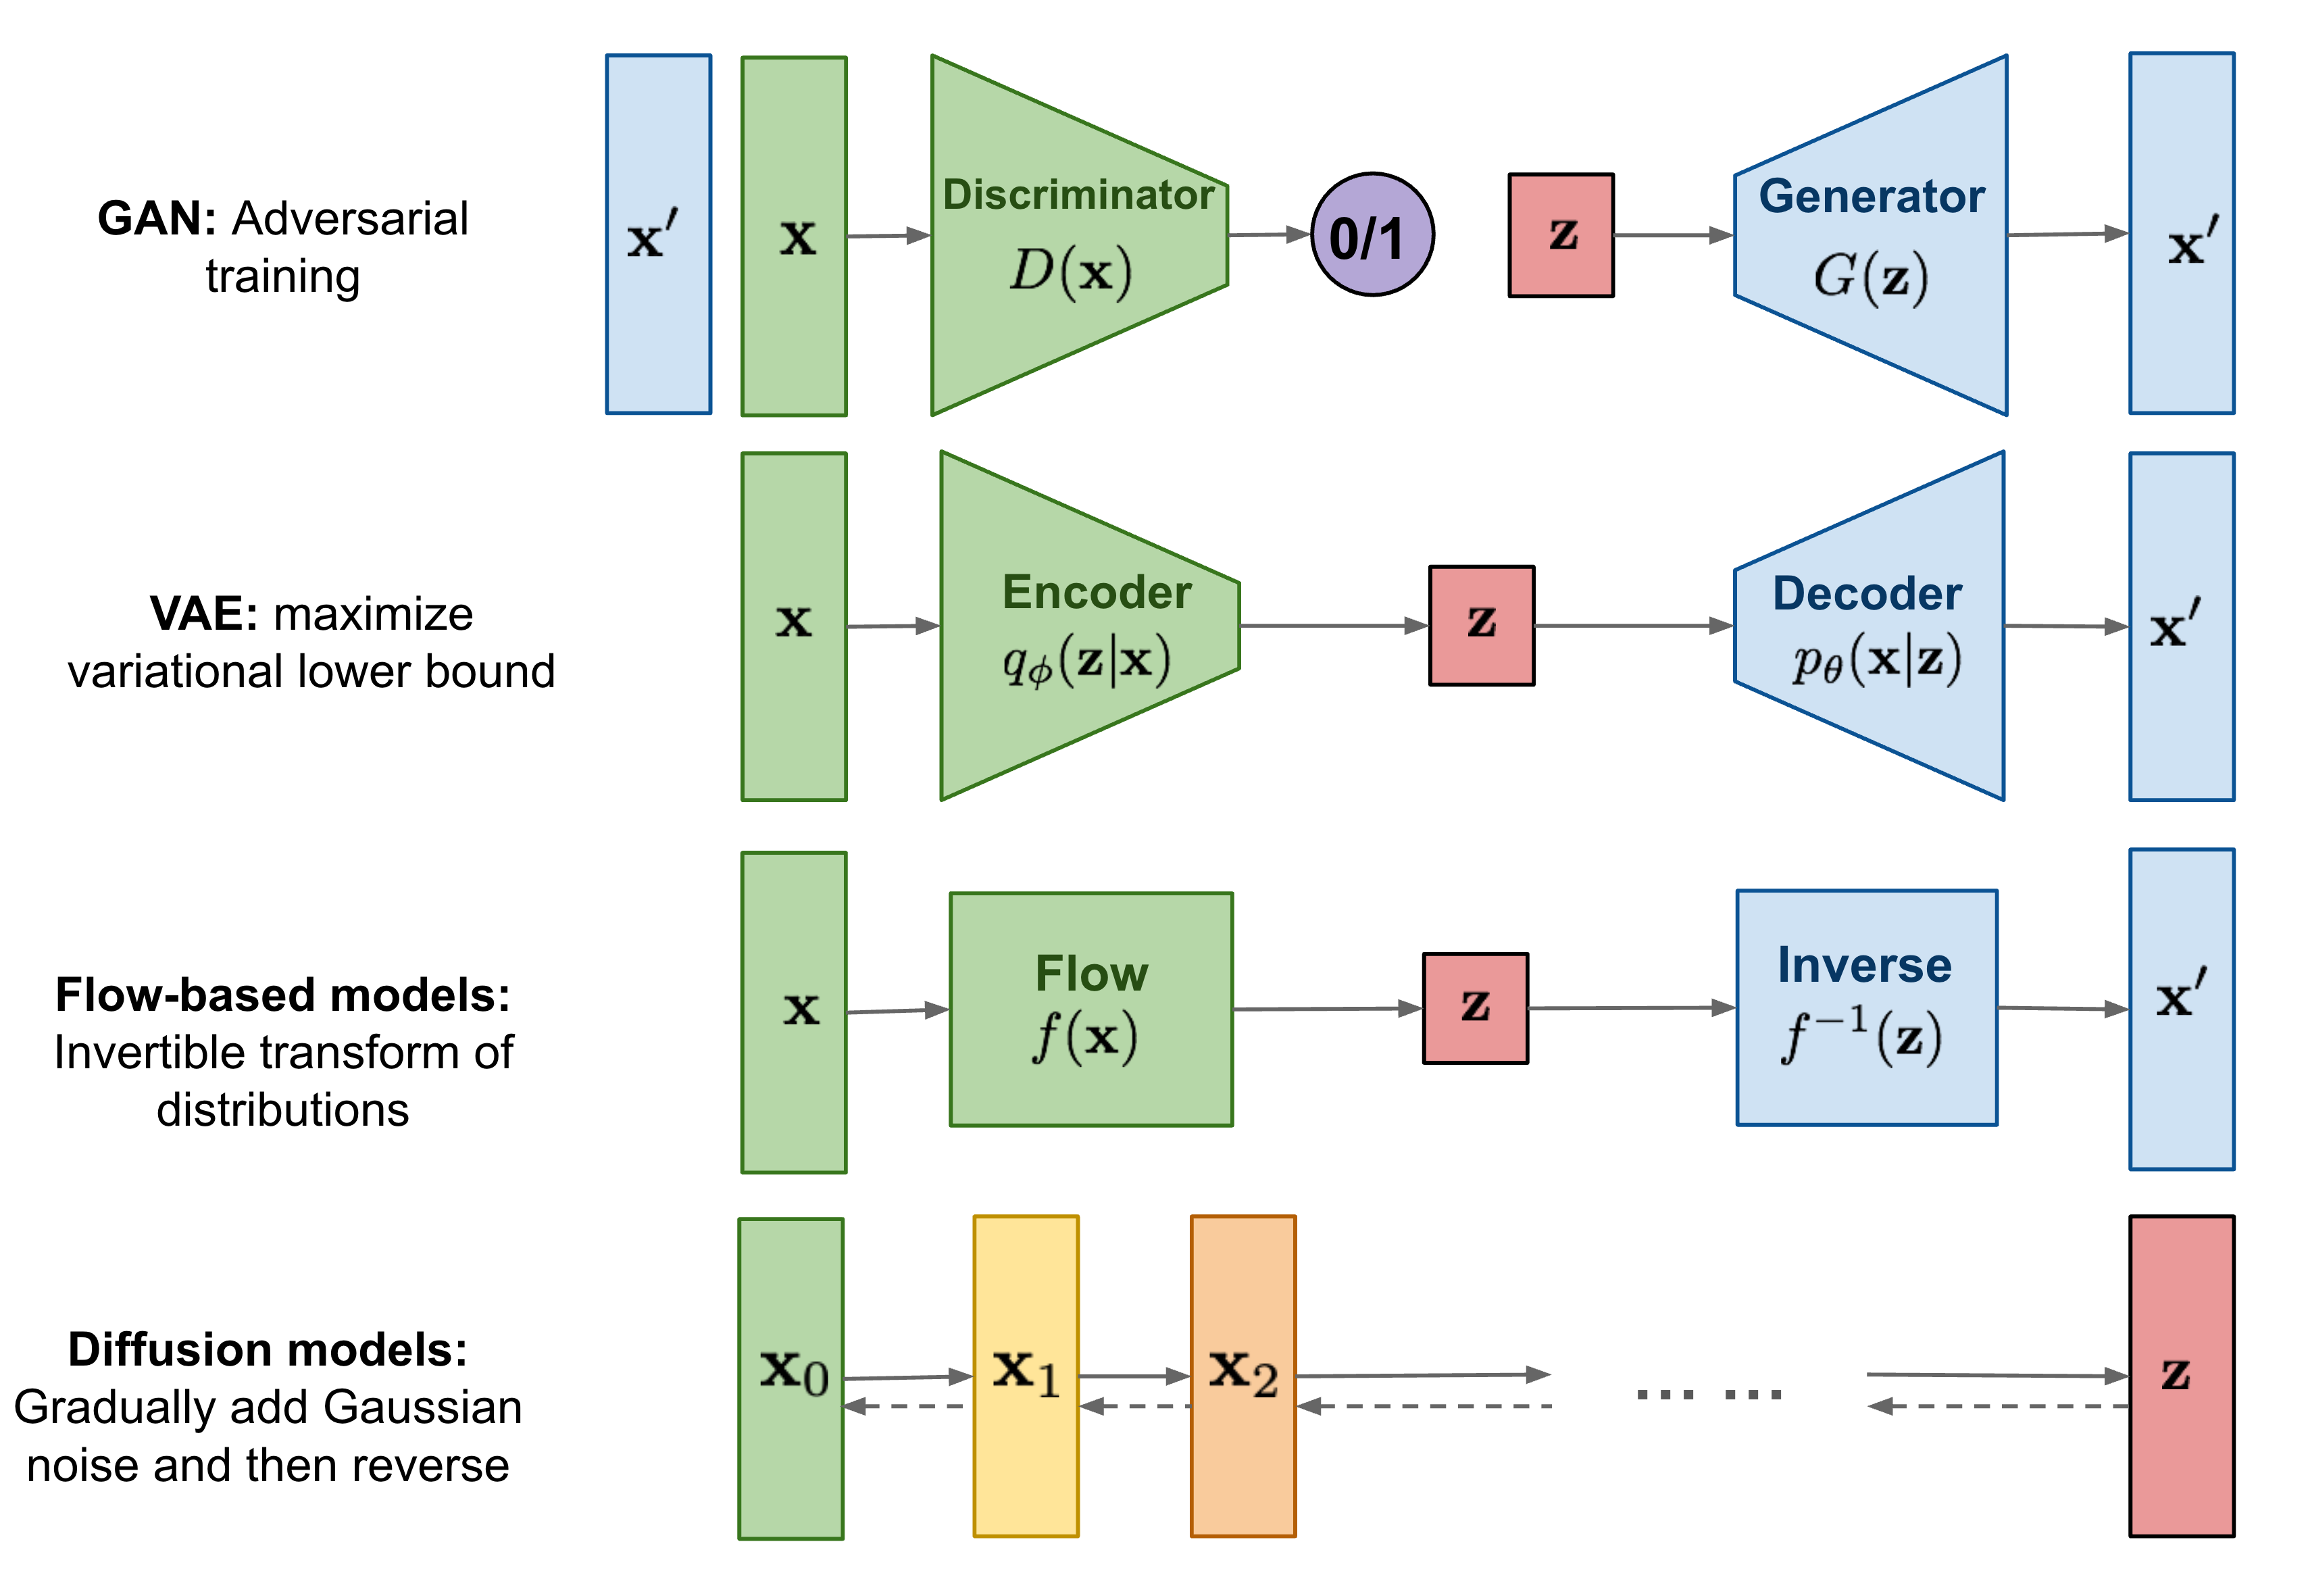
\includegraphics[width=0.9\textwidth]{generative-overview.png}
        \caption{Tổng quan các mô hình sinh}
    \end{figure}
\end{frame}

\begin{frame}

    Quá trình khuếch tán gồm hai quá trình:
    \begin{itemize}
        \item Quá trình khuếch tán thuận: nhiễu được từ từ thêm vào dữ liệu qua từng bước cho đến khi dữ liệu trở thành nhiễu có phân phối Gaussian tiêu chuẩn
        \item Quá trình khuếch tán ngược (quá trình khử nhiễu): sử dụng một mô hình được huấn luyện đảo ngược quá trình thuận (từ nhiễu trở thành dữ liệu)
    \end{itemize}
    \begin{figure}[h!]
        \centering
        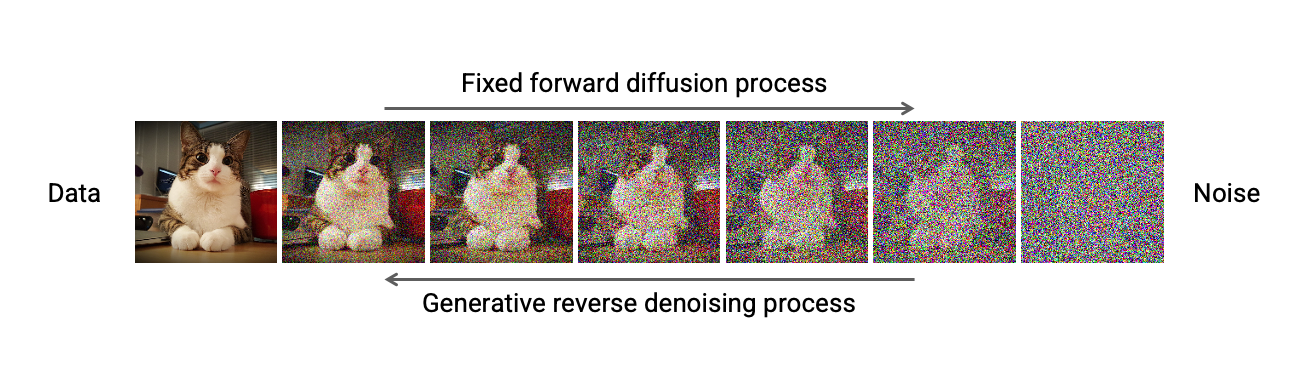
\includegraphics[width=0.9\textwidth]{Fixed_Forward_Diffusion_Process.png}
        \caption{Minh họa một quá trình khuếch tán thuận và khuếch tán ngược}
    \end{figure}
\end{frame}

\begin{frame}
    \begin{table}[h!]
        \caption{Các ký hiệu được sử dụng trong đề tài}
        \resizebox{\columnwidth}{!}{
        \begin{tabular} [c c c] {m{4cm}  m{2.5cm}  m{8cm}}
            \hline
            \multirow{5}{4cm}{Quá trình khuếch tán thuận} & $\overline{\alpha}_n, \overline{\beta}_n$ & Biểu diễn tích lũy của nhiễu Gaussian tại bước thứ $n$, $q(\boldsymbol{x}_n \vert \boldsymbol{x}_0)=\mathcal{N} \big( \boldsymbol{x}_n \vert \sqrt{\overline{\alpha}_n} \boldsymbol{x}_0, \overline{\beta}_n \boldsymbol{I} \big)$ \\ \cline{2-3}
            & $\lambda_n^2$ & Biểu diễn phương sai của quá trình khuếch tán ngược $q(\boldsymbol{x}_{n-1} \vert \boldsymbol{x}_n, \boldsymbol{x}_0)$ \\ \cline{2-3}
            & $\tilde{\boldsymbol{\mu}}_n (\boldsymbol{x}_n, \boldsymbol{x}_0)$ & Biểu diễn trung bình của quá trình khuếch tán ngược $q(\boldsymbol{x}_{n-1} \vert \boldsymbol{x}_n, \boldsymbol{x}_0)$ \\ \cline{2-3}
            & $\gamma_n$ & Biểu diễn hệ số của $\boldsymbol{x}_0$ trong $\tilde{\boldsymbol{\mu}}_n (\boldsymbol{x}_n, \boldsymbol{x}_0)$ \\ \cline{2-3}
            & $\alpha_n, \beta_n$ & Biểu diễn lượng nhiễu Gaussian được thêm vào tại từng bước $n$ trong quá trình khuếch tán thuận, $q(\boldsymbol{x}_n \vert \boldsymbol{x}_{n-1})=\mathcal{N}\big( \boldsymbol{x}_n \vert \sqrt{\alpha_n} \boldsymbol{x}_{n-1}, \beta_n \boldsymbol{I} \big)$ \\
            \hline
            \multirow{2}{4cm}{Trung bình của quá trình khuếch tán ngược} & $\boldsymbol{\mu}_n (\boldsymbol{x}_n), \boldsymbol{\mu}_n^{\ast} (\boldsymbol{x}_n)$ & Biểu diễn trung bình của quá trình khuếch tán ngược $p(\boldsymbol{x}_{n-1} \vert \boldsymbol{x}_n)$ và trung bình tối ưu \\ \cline{2-3}
            & $\hat{\boldsymbol{\epsilon}}_n (\boldsymbol{x}_n), \hat{\boldsymbol{\mu}}_n (\boldsymbol{x}_n)$ & Biểu diễn mạng dự đoán nhiễu và ước lượng của $\boldsymbol{\mu}_n^{\ast} (\boldsymbol{x}_n)$ \\
            \hline
            \multirow{4}{4cm}{Ma trận hiệp phương sai của quá trình khuếch tán ngược} & $\boldsymbol{\Sigma}_n (\boldsymbol{x}_n), \boldsymbol{\sigma}_n^{\ast} (\boldsymbol{x}_n)^2$ & Biểu diễn ma trận hiệp phương sai của quá trình khuếch tán ngược và ma trận hiệp phương sai đường chéo tối ưu \\ \cline{2-3}
            & $\boldsymbol{h}_n (\boldsymbol{x}_n), \hat{\boldsymbol{\sigma}}_n (\boldsymbol{x}_n)^2$ & Biểu diễn mạng dự đoán nhiễu bình phương SN và ước lượng của ma trận hiệp phương sai đường chéo tối ưu $\boldsymbol{\sigma}_n^{\ast} (\boldsymbol{x}_n)^2$ \\ \cline{2-3}
            & $\tilde{\boldsymbol{\sigma}}_n^{\ast} (\boldsymbol{x}_n)^2$ & Biểu diễn ma trận hiệp phương sai đường chéo tối ưu với một trung bình không hoàn hảo \\ \cline{2-3}
            & $\boldsymbol{g}_n (\boldsymbol{x}_n), \hat{\tilde{\boldsymbol{\sigma}}}_n^{\ast} (\boldsymbol{x}_n)^2$ & Biểu diễn mạng dự đoán phần dư NPR và ước lượng của $\tilde{\boldsymbol{\sigma}}_n^{\ast} (\boldsymbol{x}_n)^2$ \\
            \hline
        \end{tabular}
        }
    \end{table}
\end{frame}

\begin{frame}
    Mô hình toán học của quá trình khuếch tán thuận:
    Cho một dãy các giá trị $\beta_1, \beta_2, \hdots, \beta_N \in (0, 1)$ là một dãy tăng (thường được đặt trước). $\alpha_n = 1 - \beta_n$. $\overline{\alpha}_n = \alpha_1 \alpha_2 \hdots \alpha_n$. $\overline{\beta}_n = 1 - \overline{\alpha}_n$

    \begin{equation}
        q(\boldsymbol{x}_{1:N}\vert \boldsymbol{x}_0) = \prod_{n=1}^N q(\boldsymbol{x}_{n} \vert \boldsymbol{x}_{n-1})
    \end{equation}

    \begin{equation} \label{eq:Forward-Process}
        q\big(\boldsymbol{x}_{1:N} \vert \boldsymbol{x}_0 \big)=q\big( \boldsymbol{x}_N \vert \boldsymbol{x}_0 \big) \prod_{n=2}^{N} q\big( \boldsymbol{x}_{n-1} \vert \boldsymbol{x}_n, \boldsymbol{x}_0 \big)
    \end{equation}

    Quá trình khuếch tán thuận của DDPM là một quá trình Markov với chuyển tiếp Gaussian tuyến tính:

    \begin{equation}
        q\big( \boldsymbol{x}_n \vert \boldsymbol{x}_{n-1} \big)=\mathcal{N} \big( \boldsymbol{x}_n \vert \sqrt{\alpha}_n \boldsymbol{x}_{n-1}, \beta_n \boldsymbol{I} \big)
    \end{equation}

    Sử dụng thủ thuật tái tham số hóa:

    \begin{equation}
        \boldsymbol{x}_n = \sqrt{\alpha_n} \boldsymbol{x}_{n-1} + \sqrt{\beta_n} \boldsymbol{\epsilon} \text{ với } \boldsymbol{\epsilon} \sim \mathcal{N} (\boldsymbol{\epsilon} \vert \boldsymbol{0}, \boldsymbol{I})
    \end{equation}

    

\end{frame}

\begin{frame}
    Sử dụng tính chất cộng của hai biến ngẫu nhiên độc lập theo phân phối Gaussian tiêu chuẩn:

    \begin{equation}
        \boldsymbol{x}_n = \sqrt{\overline{\alpha}_n} \boldsymbol{x}_0 + \sqrt{\overline{\beta}_n} \boldsymbol{\epsilon}_n \text{ với } \boldsymbol{\epsilon}_n \sim \mathcal{N}(\boldsymbol{0}, \boldsymbol{I})
    \end{equation}

    \begin{equation}
        q\big( \boldsymbol{x}_n \vert \boldsymbol{x}_0 \big)=\mathcal{N} \big( \boldsymbol{x}_n \vert \sqrt{\overline{\alpha}_n} \boldsymbol{x}_0, \overline{\beta}_n \boldsymbol{I} \big)
    \end{equation}
\end{frame}

\begin{frame}
    Quá trình khuếch tán ngược:

    \begin{equation} \label{eq:Reverse-Process}
        p\big(\boldsymbol{x}_{0:N}\big)=p\big(\boldsymbol{x}_N\big)\prod_{n=1}^N p\big(\boldsymbol{x}_{n-1} \vert \boldsymbol{x}_n\big)
    \end{equation}
    với
    \begin{equation}
        p\big(\boldsymbol{x}_{n-1} \vert \boldsymbol{x}_n \big)=\mathcal{N} \big( \boldsymbol{x}_{n-1} \vert \boldsymbol{\mu}_n \big( \boldsymbol{x}_n \big), \boldsymbol{\Sigma}_n \big( \boldsymbol{x}_n \big) \big)
    \end{equation}

    Sử dụng quy tắc Bayes, ta thu được quá trình khuếch tán ngược thực sự từ quá trình tán thuận:

    \begin{equation} \label{eq:Groundtruth-Reverse-Process}
        q\big( \boldsymbol{x}_{n-1} \vert \boldsymbol{x}_n, \boldsymbol{x}_0 \big)=\mathcal{N} \big( \boldsymbol{x}_{n-1} \vert \tilde{\boldsymbol{\mu}}_n (\boldsymbol{x}_n, \boldsymbol{x}_0), \lambda_n^2 \boldsymbol{I} \big)
    \end{equation}

    \begin{equation}
        \tilde{\boldsymbol{\mu}}_n \big( \boldsymbol{x}_n, \boldsymbol{x}_0 \big)=\sqrt{\overline{\alpha}_{n-1}}\boldsymbol{x}_0 + \sqrt{\overline{\beta}_{n-1} - \lambda_n^2}.\dfrac{\boldsymbol{x}_n - \sqrt{\overline{\alpha}_n}\boldsymbol{x}_0}{\sqrt{\overline{\beta}_n}}
    \end{equation}

    \begin{equation}
        \lambda_n = \dfrac{\overline{\beta}_{n-1}}{\overline{\beta}_n}\beta_n \text{ (DDPM) \cite{ho2020denoising} và } \lambda_n = 0 \text{ DDIM \cite{song2020denoising}}
    \end{equation}
\end{frame}

\begin{frame}
    Quá trình khuếch tán ngược được học bằng cách cực đại hóa cận dưới (ELBO): $L_{\mathrm{elbo}}=\mathbb{E}_q \log \dfrac{p(\boldsymbol{x}_{0:N})}{q(\boldsymbol{x}_{1:N}\vert \boldsymbol{x}_0)}$ hay tương đương với cực tiểu hóa độ phân kỳ Kullback-Leibler giữa quá trình khuếch tán thuận và quá trình khuếch tán ngược:

    \begin{equation} \label{eq:ELBO-Maximization}
        \max_{\lbrace \boldsymbol{\mu}_n, \boldsymbol{\Sigma}_n \rbrace_{n=1}^N} L_{\mathrm{elbo}} \Leftrightarrow \min_{\lbrace \boldsymbol{\mu}_n, \boldsymbol{\Sigma}_n \rbrace_{n=1}^N} D_{\mathrm{KL}} \big( q(\boldsymbol{x}_{0:N}) \Vert p(\boldsymbol{x}_{0:N}) \big)
    \end{equation}
\end{frame}


\begin{frame}
    \begin{algorithm}[H]
        \DontPrintSemicolon
        \KwIn{Mạng dự đoán nhiễu $\hat{\boldsymbol{\epsilon}}_n (\boldsymbol{x}_n)$ và tham số được huấn luyện $\boldsymbol{\theta}$}
        \Repeat{hội tụ}{
            $\boldsymbol{x}_0 \sim q(\boldsymbol{x}_0)$\;
            $n \sim \mathrm{Uniform}\big( \lbrace 1, 2, \dots, N \rbrace\big)$\;
            $\boldsymbol{\epsilon} \sim \mathcal{N}(\boldsymbol{0}, \boldsymbol{I})$\;
            $\boldsymbol{x}_n \gets \sqrt{\overline{\alpha}_n} \boldsymbol{x}_0 + \sqrt{\overline{\beta}_n} \boldsymbol{\epsilon}$\;
            Chỉnh định $\boldsymbol{\theta}$ dựa trên đạo hàm riêng $\nabla_{\boldsymbol{\theta}}  \lVert \boldsymbol{\epsilon}^2 - \hat{\boldsymbol{\epsilon}}_n (\boldsymbol{x}_n) \rVert_2^2$
        }
        \caption{Thủ tục huấn luyện VDM}
        \label{alg:Learning-of-VDM}
    \end{algorithm}
\end{frame}

\begin{frame}
    \begin{algorithm}[H]
        \DontPrintSemicolon
        \KwIn{Mạng dự đoán nhiễu $\hat{\boldsymbol{\epsilon}}_n (\boldsymbol{x}_n)$ và tham số đã được huấn luyện $\boldsymbol{\theta}$}
        $\boldsymbol{x}_N \sim \mathcal{N} (\boldsymbol{0}, \boldsymbol{I})$\;
        \For {$t \gets N, \dots, 1$} {
            \If {$n > 1$} {
                $\boldsymbol{\epsilon} \sim \mathcal{N}(\boldsymbol{0}, \boldsymbol{I})$\;
            } \Else {
                $\boldsymbol{\epsilon} \gets \boldsymbol{0}$\;
            }
        $\boldsymbol{x}_{n-1} \gets \dfrac{1}{\sqrt{\alpha_n}} \Big( \boldsymbol{x}_n - \dfrac{1 - \alpha_n}{\sqrt{1 - \overline{\alpha}_n}} \hat{\boldsymbol{\epsilon}}_n (\boldsymbol{x}_n) \Big) + \lambda_n \boldsymbol{\epsilon}$\;
        }
        \Return{$\boldsymbol{x}_0$}\;
        \caption{Thủ tục lấy mẫu từ một VDM đã được huấn luyện}
        \label{alg:Sampling-of-VDM}
    \end{algorithm}
\end{frame}

\begin{frame}
    Khi sử dụng ma trận đẳng hướng, \cite{bao2021analytic} đã chỉ ra cả trung bình tối ưu $\boldsymbol{\mu}_n^{\ast} (\boldsymbol{x}_n)$ và phương sai tối ưu có dạng giải tích tương ứng với kỳ vọng có điều kiện của nhiễu $\mathbb{E}_{q( \boldsymbol{x}_0 \vert \bold{x}_n )} \lbrack \boldsymbol{\epsilon}_n \rbrack$:

    \begin{equation} \label{eq:Optimal-Mean}
        \boldsymbol{\mu}_n^{\ast} (\boldsymbol{x}_n)=\tilde{\boldsymbol{\mu}}_n \Bigg( \boldsymbol{x}_n, \dfrac{1}{\sqrt{\overline{\alpha}_n}} \Big( \boldsymbol{x}_n - \sqrt{\overline{\beta}_n} \mathbb{E}_{q(\boldsymbol{x}_0 \vert \boldsymbol{x}_n)} \lbrack \boldsymbol{\epsilon}_n \rbrack \Big) \Bigg)
    \end{equation}

    \begin{equation} \label{eq:Optimal-Isotropic-Variance}
        \sigma_n^{\ast 2}=\lambda_n^2 + \gamma_n^2 \dfrac{\overline{\beta}_n}{\overline{\alpha}_n} \Bigg( 1 - \mathbb{E}_{q(\boldsymbol{x}_n)} \dfrac{\lVert \mathbb{E}_{q(\boldsymbol{x}_0 \vert \boldsymbol{x}_n)} \lbrack \boldsymbol{\epsilon}_n \rbrack\rVert_2^2}{d} \Bigg)
    \end{equation}
\end{frame}

\begin{frame}

    \cite{ho2020denoising} ước lượng $\boldsymbol{\mu}_n^{\ast} (\boldsymbol{x}_n)$ sử dụng một mạng dự đoán nhiễu $\hat{\boldsymbol{\epsilon}}_n (\boldsymbol{x}_n)$:
    \begin{equation} \label{eq:Estimated-Optimal-Mean}
        \hat{\boldsymbol{\mu}}_n(\boldsymbol{x}_n)=\tilde{\boldsymbol{\mu}}_n \Bigg( \boldsymbol{x}_n, \dfrac{1}{\sqrt{\overline{\alpha}_n}} \Big( \bold{x}_n - \sqrt{\overline{\beta}_n} \hat{\boldsymbol{\epsilon}}_n(\boldsymbol{x}_n) \Big) \Bigg)
    \end{equation}

    Mạng $\hat{\boldsymbol{\epsilon}}_n (\boldsymbol{x}_n)$ cần phải học được kỳ vọng $\mathbb{E}_{q( \boldsymbol{x}_0 \vert \bold{x}_n )} \lbrack \boldsymbol{\epsilon}_n \rbrack$ bằng cách cực tiểu hóa hàm mục tiêu MSE:

    \begin{equation} \label{eq:Noise-Prediction}
        \min_{\lbrace \hat{\boldsymbol{\epsilon}}_n  \rbrace_{n=1}^N} \mathbb{E}_n  \mathbb{E}_{q(\boldsymbol{x}_0, \boldsymbol{x}_n)} \lVert \boldsymbol{\epsilon}_n - \hat{\boldsymbol{\epsilon}}_n (\boldsymbol{x}_n) \rVert_2^2
    \end{equation}
\end{frame}

\begin{frame}
    \begin{dl}[Nghiệm tối ưu cho bài toán tối ưu hóa chung] \label{dl:Optimal-Solution-To-Joint-Optimization}
        Với ma trận hiệp phương sai có dạng $\boldsymbol{\Sigma}_n (\boldsymbol{x}_n)=\mathrm{diag}\big( \boldsymbol{\sigma}_n (\boldsymbol{x}_n)^2 \big)$.
        Khi đó trung bình tối ưu của bài toán trong công thức \ref{eq:ELBO-Maximization} là $\boldsymbol{\mu}_n^{\ast} (\boldsymbol{x}_n)$ được nêu trong công thức \ref{eq:Optimal-Mean},
        và ma trận hiệp phương sai tối ưu của bài toán trong công thức \ref{eq:ELBO-Maximization} là:

        \begin{equation*}
            \boldsymbol{\sigma}_n^{\ast} (\boldsymbol{x}_n)^2 = \lambda_n^2 \boldsymbol{1} + \gamma_n^2 \dfrac{\overline{\beta}_n}{\overline{\alpha}_n} \big( \mathbb{E}_{q(\boldsymbol{x}_0 \vert \boldsymbol{x}_n)} \lbrack \boldsymbol{\epsilon}_n^2 \rbrack - \mathbb{E}_{q(\boldsymbol{x}_0 \vert \boldsymbol{x}_n)} \lbrack \boldsymbol{\epsilon}_n \rbrack^2 \big)
        \end{equation*}
        với $\boldsymbol{\epsilon}_n = \dfrac{\boldsymbol{x}_n - \sqrt{\overline{\alpha}_n} \boldsymbol{x}_0}{\sqrt{\overline{\beta}_n}}$ là nhiễu được dùng để tạo ra $\boldsymbol{x}_n$ từ $\boldsymbol{x}_0$,
        $(.)^2$ là bình phương từng phần tử của vector, $\boldsymbol{1}$ là vector mà các phần tử đều bằng một và $\gamma_n = \sqrt{\overline{\alpha}_{n-1}} - \sqrt{\overline{\beta}_{n-1} - \lambda_n^2} \sqrt{\dfrac{\overline{\alpha}_n}{\overline{\beta}_n}}$
    \end{dl}
\end{frame}


\begin{frame}
    Để ước lượng ma trận hiệp phương sai tối ưu $\boldsymbol{\sigma}_n^{\ast} (\boldsymbol{x}_n)^2$ trong định lý \ref{dl:Optimal-Solution-To-Joint-Optimization}, ta cần phải ước lượng cả hai đại lượng $\mathbb{E}_{q(\boldsymbol{x}_0 \vert \boldsymbol{x}_n)} \lbrack \boldsymbol{\epsilon}_n \rbrack^2$ và $\mathbb{E}_{q(\boldsymbol{x}_0 \vert \boldsymbol{x}_n)} \lbrack \boldsymbol{\epsilon}_n^2 \rbrack$.
    
    Mạng dự đoán nhiễu $\hat{\boldsymbol{\epsilon}}_n (\boldsymbol{x}_n)$ có mục đích ước lượng $\mathbb{E}_{q(\boldsymbol{x}_0 \vert \boldsymbol{x}_n)} \lbrack \boldsymbol{\epsilon}_n \rbrack$ bằng cách cực tiểu hóa hàm mục tiêu MSE trong công thức \ref{eq:Noise-Prediction}.

    $\hat{\boldsymbol{\epsilon}}_n (\boldsymbol{x}_n)^2$ để ước lượng $\mathbb{E}_{q(\boldsymbol{x}_0 \vert \boldsymbol{x}_n)} \lbrack \boldsymbol{\epsilon}_n \rbrack^2$.
\end{frame}

\begin{frame}
    $\mathbb{E}_{q(\boldsymbol{x}_0 \vert \boldsymbol{x}_n)} \lbrack \boldsymbol{\epsilon}_n^2 \rbrack$ là kỳ vọng có điều kiện của bình phương của nhiễu (SN) $\boldsymbol{\epsilon}_n^2$ điều kiện trên $\boldsymbol{x}_n$.

    Đại lượng kỳ vọng này có thể được ước lượng sử dụng mạng $\boldsymbol{h}_n (\boldsymbol{x}_n) \in \mathbb{R}^d$ được huấn luyện trên hàm mục tiêu MSE:

    \begin{equation} \label{eq:Square-Noise-Prediction-Network-MSE-Loss}
        \min_{\lbrace \boldsymbol{h}_n \rbrace_{n=1}^N} \mathbb{E}_n \mathbb{E}_{q(\boldsymbol{x}_0, \boldsymbol{x}_n)} \lVert \boldsymbol{\epsilon}_n^2 - \boldsymbol{h}_n (\boldsymbol{x}_n) \rVert_2^2
    \end{equation}

    $\boldsymbol{h}_n (\boldsymbol{x}_n)$ là mạng dự đoán nhiễu bình phương (SN).

    Bằng cách ước lượng $\mathbb{E}_{q(\boldsymbol{x}_0 \vert \boldsymbol{x}_n)} \lbrack \boldsymbol{\epsilon}_n \rbrack^2$ với $\hat{\boldsymbol{\epsilon}}_n (\boldsymbol{x}_n)^2$ và $\mathbb{E}_{q(\boldsymbol{x}_0 \vert \boldsymbol{x}_n)} \lbrack \boldsymbol{\epsilon}_n^2 \rbrack$ với $\boldsymbol{h}_n (\boldsymbol{x}_n)$,
    ta có thể ước lượng:

    \begin{equation} \label{eq:Sigma-SN-SPM}
        \hat{\boldsymbol{\sigma}}_n (\boldsymbol{x}_n)^2 = \lambda_n^2 \boldsymbol{1} + \gamma_n^2 \dfrac{\overline{\beta}_n}{\overline{\alpha}_n} \big( \boldsymbol{h}_n (\boldsymbol{x}_n) - \hat{\boldsymbol{\epsilon}}_n (\boldsymbol{x}_n)^2 \big)
    \end{equation}
\end{frame}

\begin{frame}
    \begin{algorithm}[H]
        \DontPrintSemicolon
        \KwIn{Mạng dự đoán bình phương nhiễu (SN) $\boldsymbol{h}_n (\boldsymbol{x}_n)$ và tham số được huấn luyện $\boldsymbol{\phi}_2$}
        \Repeat{hội tụ}{
            $\boldsymbol{x}_0 \sim q(\boldsymbol{x}_0)$\;
            $n \sim \mathrm{Uniform}\big( \lbrace 1, 2, \dots, N \rbrace\big)$\;
            $\boldsymbol{\epsilon}_n \sim \mathcal{N}(\boldsymbol{0}, \boldsymbol{I})$\;
            $\boldsymbol{x}_n \gets \sqrt{\overline{\alpha}_n} \boldsymbol{x}_0 + \sqrt{\overline{\beta}_n} \boldsymbol{\epsilon}_n$\;
            Chỉnh định $\boldsymbol{\phi}_2$ dựa trên đạo hàm riêng $\nabla_{\boldsymbol{\phi}_2}  \lVert \boldsymbol{\epsilon}_n^2 - \boldsymbol{h}_n (\boldsymbol{x}_n) \rVert_2^2$
        }
        \caption{Thủ tục huấn luyện mạng dự đoán nhiễu bình phương (SN)}
        \label{alg:Learning-of-the-SN-prediction-network}
    \end{algorithm}
\end{frame}

\begin{frame}
    \begin{algorithm}[H]
        \DontPrintSemicolon
        \KwIn{Mạng dự đoán nhiễu $\hat{\boldsymbol{\epsilon}}_n (\boldsymbol{x}_n)$ với tham số $\boldsymbol{\phi}_1$ và mạng dự đoán bình phương nhiễu (SN) $\boldsymbol{h}_n (\boldsymbol{x}_n)$ với tham số $\boldsymbol{\phi}_2$}
        $\boldsymbol{x}_N \sim \mathcal{N} (\boldsymbol{0}, \boldsymbol{I})$\;
        \For {$t \gets N, \dots, 1$} {
            \If {$n > 1$} {
                $\boldsymbol{\epsilon} \sim \mathcal{N}(\boldsymbol{0}, \boldsymbol{I})$\;
            } \Else {
                $\boldsymbol{\epsilon} \gets \boldsymbol{0}$\;
            }
            $\hat{\boldsymbol{\sigma}}_n (\boldsymbol{x}_n)^2 \gets \lambda_n^2 \boldsymbol{1} + \gamma_n^2 \dfrac{\overline{\beta}_n}{\overline{\alpha}_n} \big( \boldsymbol{h}_n (\boldsymbol{x}_n) - \hat{\boldsymbol{\epsilon}}_n (\boldsymbol{x}_n)^2 \big)$\;
        $\boldsymbol{x}_{n-1} \gets \dfrac{1}{\sqrt{\alpha_n}} \Big( \boldsymbol{x}_n - \dfrac{1 - \alpha_n}{\sqrt{1 - \overline{\alpha}_n}} \hat{\boldsymbol{\epsilon}}_n (\boldsymbol{x}_n) \Big) + \hat{\boldsymbol{\sigma}}_n (\boldsymbol{x}_n) \odot \boldsymbol{\epsilon}$\;
        }
        \Return{$\boldsymbol{x}_0$}\;
        \caption{Thủ tục lấy mẫu từ một SN-DPM đã được huấn luyện}
        \label{alg:Sampling-of-SN}
    \end{algorithm}
\end{frame}

\begin{frame}
    Không thể tính toán chính xác hai đại lương $\boldsymbol{\mu}_n^{\ast} (\boldsymbol{x}_n)$ và $\boldsymbol{\sigma}_n^{\ast} (\boldsymbol{x}_n)^2$ do có thành phần kỳ vọng có điều kiện trên hàm của nhiễu $\mathbb{E}_{q(\boldsymbol{x}_0 \vert \boldsymbol{x}_n)} \lbrack \boldsymbol{\epsilon}_n \rbrack$.


    Một cách tự nhiên, ta sẽ tối ưu duy nhất trung bình để thu được ước lượng của trung bình tối ưu $\hat{\boldsymbol{\mu}}_n$ và sau đó với tối ưu ma trận hiệp phương sai khi đã biết trung bình tối ưu $\hat{\boldsymbol{\mu}}_n$:

    \begin{equation}
        L_{\mathrm{elbo}}\big( \hat{\boldsymbol{\mu}}_n, \hat{\boldsymbol{\sigma}}_n (\boldsymbol{x}_n)^2 \big) \leq \max_{\boldsymbol{\sigma}_n (.)^2 } L_{\mathrm{elbo}} \big( \hat{\boldsymbol{\mu}}_n, \boldsymbol{\sigma}_n (.)^2 \big)
    \end{equation}

    Và dấu bằng về cơ bản không xảy ra.
\end{frame}

\begin{frame}
    Ta thu được các lời giải tối ưu bằng cách giải hai bài toán:

    \begin{equation} \label{eq:Arbitrary-Covariance-Optimize-Mean}
        \text{Cho ma trận hiệp phương sai bất kỳ } \boldsymbol{\Sigma}_n, \max_{\lbrace \boldsymbol{\mu}_n \rbrace_{n=1}^N} L_{\mathrm{elbo}}
    \end{equation}

    \begin{equation} \label{eq:Arbitrary-Mean-Optimize-Covariance}
        \text{Cho trung bình bất kỳ } \boldsymbol{\mu}_n, \max_{\lbrace \boldsymbol{\Sigma}_n \rbrace_{n=1}^N} L_{\mathrm{elbo}}
    \end{equation}
\end{frame}


\begin{frame}
    \begin{dl}[Lời giải tối ưu của bài toán tối ưu duy nhất với trung bình] \label{dl:Solely-Optimal-Mean}
        Với ma trận hiệp phương sai bất kỳ $\boldsymbol{\Sigma}_n$,
        trung bình tối ưu của bài toán trong công thức \ref{eq:Arbitrary-Covariance-Optimize-Mean} luôn luôn là trung bình tối ưu trong công thức \ref{eq:Optimal-Mean}:

        \begin{equation*}
            \boldsymbol{\mu}_n^{\ast} (\boldsymbol{x}_n)=\tilde{\boldsymbol{\mu}}_n \Bigg( \boldsymbol{x}_n, \dfrac{1}{\sqrt{\overline{\alpha}_n}} \Big( \boldsymbol{x}_n - \sqrt{\overline{\beta}_n} \mathbb{E}_{q(\boldsymbol{x}_0 \vert \boldsymbol{x}_n)} \lbrack \boldsymbol{\epsilon}_n \rbrack \Big) \Bigg)
        \end{equation*}

        không ảnh hưởng đến $\boldsymbol{\Sigma}_n$.
    \end{dl}
\end{frame}



\begin{frame}
    \begin{dl}[Lời giải tối ưu của bài toán tối ưu duy nhất với ma trận hiệp phương sai] \label{dl:Solely-Optimal-Covariance}
        Ta giả định $\boldsymbol{\Sigma}_n = \mathrm{diag} \big( \boldsymbol{\sigma}_n (\boldsymbol{x}_n)^2 \big)$.
        Với trung bình bất kỳ $\boldsymbol{\mu}_n (\boldsymbol{x}_n)$ được tham số hóa bởi mạng dự đoán nhiễu $\hat{\boldsymbol{\epsilon}}_n (\boldsymbol{x}_n)$ như trong công thức \ref{eq:Estimated-Optimal-Mean},
        ma trận hiệp phương sai tối ưu của bài toán trong công thức \ref{eq:Arbitrary-Mean-Optimize-Covariance} là:

        \begin{equation} \label{eq:Corrected-Optimal-Covariance}
            \begin{aligned}
                \tilde{\boldsymbol{\sigma}}_n^{\ast} (\boldsymbol{x}_n)^2 &= \boldsymbol{\sigma}_n^{\ast} (\boldsymbol{x}_n)^2 + \gamma_n^2 \dfrac{\overline{\beta}_n}{\overline{\alpha}_n} \underbrace{\big( \hat{\boldsymbol{\epsilon}}_n (\boldsymbol{x}_n) - \mathbb{E}_{q(\boldsymbol{x}_0 \vert \boldsymbol{x}_n) \lbrack \boldsymbol{\epsilon}_n \rbrack} \big)^2}_{\mathrm{error}} \\
                &= \lambda_n^2 \boldsymbol{1} + \gamma_n^2 \dfrac{\overline{\beta}_n}{\overline{\alpha}_n} \mathbb{E}_{q(\boldsymbol{x}_0 \vert \boldsymbol{x}_n)} \Big\lbrack \big( \boldsymbol{\epsilon}_n - \hat{\boldsymbol{\epsilon}}_n (\boldsymbol{x}_n) \big)^2 \Big\rbrack
            \end{aligned}
        \end{equation}

        Với $\boldsymbol{\sigma}_n^{\ast} (\boldsymbol{x}_n)^2$ là ma trận hiệp phương sai tối ưu của bài toán tối ưu hóa chung ở định lý \ref{dl:Optimal-Solution-To-Joint-Optimization},
        $\boldsymbol{\epsilon}_n = \dfrac{\boldsymbol{x}_n - \sqrt{\overline{\alpha}_n} \boldsymbol{x}_0}{\sqrt{\overline{\beta}_n}}$ là nhiễu được dùng để tạo ra $\boldsymbol{x}_n$ từ $\boldsymbol{x}_0$,
        $(.)^2$ là bình phương từng phần tử của vector, $\boldsymbol{1}$ là vector mà các phần tử đều bằng một và $\gamma_n = \sqrt{\overline{\alpha}_{n-1}} - \sqrt{\overline{\beta}_{n-1} - \lambda_n^2} \sqrt{\dfrac{\overline{\alpha}_n}{\overline{\beta}_n}}$.
    \end{dl}
\end{frame}


\begin{frame}
    Công thức \ref{eq:Corrected-Optimal-Covariance}, ma trận hiệp phương sai tối ưu đã được hiệu chỉnh $\tilde{\boldsymbol{\sigma}}_n^{\ast} (\boldsymbol{x}_n)^2$ được xác định qua $\mathbb{E}_{q(\boldsymbol{x}_0 \vert \boldsymbol{x}_n)} \Big\lbrack \big( \boldsymbol{\epsilon}_n - \hat{\boldsymbol{\epsilon}}_n (\boldsymbol{x}_n) \big)^2 \Big\rbrack$.
    
    Ta học đại lượng này bằng cách huấn luyện một mạng $\boldsymbol{g}_n (\boldsymbol{x}_n) \in \mathbb{R}^d$ dự đoán $\big( \boldsymbol{\epsilon}_n - \hat{\boldsymbol{\epsilon}}_n (\boldsymbol{x}_n) \big)^2$ khi biết $\boldsymbol{x}_n$ bằng cách cực tiểu hóa hàm mục tiêu MSE:

    \begin{equation} \label{eq:Square-Noise-Residual-Prediction-Network-MSE-Loss}
        \min_{\lbrace \boldsymbol{g}_n \rbrace_{n=1}^N} \mathbb{E}_n \mathbb{E}_{q(\boldsymbol{x}_0, \boldsymbol{x}_n)} \lVert \big( \boldsymbol{\epsilon}_n - \hat{\boldsymbol{\epsilon}}_n (\boldsymbol{x}_n) \big)^2 - \boldsymbol{g}_n (\boldsymbol{x}_n)  \rVert_2^2
    \end{equation}

    Với $n$ được lấy mẫu theo phân phối đều từ $\lbrace 1, 2, \dots, N \rbrace$.
\end{frame}

\begin{frame}
    Với mạng dự đoán phần dư nhiễu $\boldsymbol{g}_n (\boldsymbol{x}_n)$ trong công thức \ref{eq:Square-Noise-Residual-Prediction-Network-MSE-Loss},
    ta ước lượng $\tilde{\boldsymbol{\sigma}}_n^{\ast} (\boldsymbol{x}_n)^2$ bằng công thức:

    \begin{equation} \label{eq:Sigma-NPR-DPM}
        \hat{\tilde{\boldsymbol{\sigma}}}_n (\boldsymbol{x}_n)^2 = \lambda_n^2 \boldsymbol{1} + \gamma_n^2 \dfrac{\overline{\beta}_n}{\overline{\alpha}_n} \boldsymbol{g}_n (\boldsymbol{x}_n)
    \end{equation}

    Trong tiểu luận ta gọi ước lượng này là SNR-DPM.
\end{frame}


\begin{frame}
    \begin{algorithm}[H]
        \DontPrintSemicolon
        \KwIn{Mạng dự đoán phần dư nhiễu (NPR) $\boldsymbol{g}_n (\boldsymbol{x}_n)$ và tham số được huấn luyện $\boldsymbol{\phi}_2$;
        mạng dự đoán nhiễu đã được tiền huấn luyện $\hat{\boldsymbol{\epsilon}}_n (\boldsymbol{x}_n)$}
        \Repeat{hội tụ}{
            $\boldsymbol{x}_0 \sim q(\boldsymbol{x}_0)$\;
            $n \sim \mathrm{Uniform}\big( \lbrace 1, 2, \dots, N \rbrace\big)$\;
            $\boldsymbol{\epsilon}_n \sim \mathcal{N}(\boldsymbol{0}, \boldsymbol{I})$\;
            $\boldsymbol{x}_n \gets \sqrt{\overline{\alpha}_n} \boldsymbol{x}_0 + \sqrt{\overline{\beta}_n} \boldsymbol{\epsilon}_n$\;
            Chỉnh định $\boldsymbol{\phi}_2$ dựa trên đạo hàm riêng $\nabla_{\boldsymbol{\phi}_2}  \lVert \big( \boldsymbol{\epsilon}_n - \hat{\boldsymbol{\epsilon}}_n (\boldsymbol{x}_n) \big)^2 - \boldsymbol{g}_n (\boldsymbol{x}_n) \rVert_2^2$
        }
        \caption{Thủ tục huấn luyện mạng dự đoán phần dư nhiễu (NPR)}
        \label{alg:Learning-of-the-NPR-prediction-network}
    \end{algorithm}
\end{frame}


\begin{frame}
    \begin{algorithm}[H]
        \DontPrintSemicolon
        \KwIn{Mạng dự đoán nhiễu $\hat{\boldsymbol{\epsilon}}_n (\boldsymbol{x}_n)$ với tham số $\boldsymbol{\phi}_1$ và mạng dự đoán phần dư nhiễu (NPR) $\boldsymbol{g}_n (\boldsymbol{x}_n)$ với tham số $\boldsymbol{\phi}_2$}
        $\boldsymbol{x}_N \sim \mathcal{N} (\boldsymbol{0}, \boldsymbol{I})$\;
        \For {$t \gets N, \dots, 1$} {
            \If {$n > 1$} {
                $\boldsymbol{\epsilon} \sim \mathcal{N}(\boldsymbol{0}, \boldsymbol{I})$\;
            } \Else {
                $\boldsymbol{\epsilon} \gets \boldsymbol{0}$\;
            }
            $\hat{\tilde{\boldsymbol{\sigma}}}_n (\boldsymbol{x}_n)^2 \gets \lambda_n^2 \boldsymbol{1} + \gamma_n^2 \dfrac{\overline{\beta}_n}{\overline{\alpha}_n} \boldsymbol{g}_n (\boldsymbol{x}_n)$\;
        $\boldsymbol{x}_{n-1} \gets \dfrac{1}{\sqrt{\alpha_n}} \Big( \boldsymbol{x}_n - \dfrac{1 - \alpha_n}{\sqrt{1 - \overline{\alpha}_n}} \hat{\boldsymbol{\epsilon}}_n (\boldsymbol{x}_n) \Big) + \hat{\tilde{\boldsymbol{\sigma}}}_n (\boldsymbol{x}_n) \odot \boldsymbol{\epsilon}$\;
        }
        \Return{$\boldsymbol{x}_0$}\;
        \caption{Thủ tục lấy mẫu từ một NPR-DPM đã được huấn luyện}
        \label{alg:Sampling-of-NPR}
    \end{algorithm}
\end{frame}

\begin{frame}
    SN-DPM và NPR-DPM cần được chạy cả hai mạng.

    Để giảm chi phí tính toán, ta sử dụng phương pháp chia sẻ tham số giữa hai mạng như sau:

    \begin{equation} \label{eq:Parameter-Sharing-Scheme}
        \begin{aligned}
        \hat{\boldsymbol{\epsilon}}_n (\boldsymbol{x}_n) &= \mathrm{NN}_1 (\mathrm{UNet}(\boldsymbol{x}_n, n ; \boldsymbol{\theta}); \boldsymbol{\phi}_1) \\
        \boldsymbol{h}_n (\boldsymbol{x}_n) \text{ hoặc } \boldsymbol{g}_n (\boldsymbol{x}_n) &= \mathrm{NN}_2(\mathrm{UNet}(\boldsymbol{x}_n, n; \boldsymbol{\theta}); \boldsymbol{\phi}_2)
        \end{aligned}
    \end{equation}

    Với $\mathrm{UNet}$ là một trong những cấu trong rất phổ biến trong DPMs \cite{ho2020denoising}, \cite{song2020score} và được tham số hóa bởi tham số được chia sẻ $\boldsymbol{\theta}$.

    $\mathrm{NN}_1$ và $\mathrm{NN}_2$ là hai mạng nhỏ bao gồm một vài lớp tích chập và được tham số hóa bởi $\boldsymbol{\phi}_1$ và $\boldsymbol{\phi}_2$ tương ứng.
\end{frame}

\begin{frame}
    Quá trình huấn luyện được chia làm hai giai đoạn:
    \begin{itemize}
        \item Trong giai đoạn đầu tiên, ta học trung bình bằng cách huấn luyện mạng dự đoán nhiễu ở công thức \ref{eq:Noise-Prediction},
        hoặc chỉ cần sử dụng một mạng đã được tiền huấn luyện từ các công trình trước.
        \item Trong giai đoạn hai, huấn luyện mạng dự đoán phương sai với tham số $\boldsymbol{\phi}_2$:

        \begin{equation}
            \begin{aligned}
            &\nabla_{\boldsymbol{\phi}_1} \mathbb{E}_n \mathbb{E}_{q(\boldsymbol{x}_0, \boldsymbol{x}_n)} \lVert \boldsymbol{\epsilon}_n^2 - \boldsymbol{h}_n (\boldsymbol{x}_n) \rVert_2^2, \text{ hoặc} \\
            &\nabla_{\boldsymbol{\phi}_2} \mathbb{E}_n \mathbb{E}_{q(\boldsymbol{x}_0, \boldsymbol{x}_n)} \lVert \big( \boldsymbol{\epsilon}_n - \hat{\boldsymbol{\epsilon}}_n (\boldsymbol{x}_n) \big)^2 - \boldsymbol{g}_n (\boldsymbol{x}_n) \rVert_2^2
            \end{aligned}
        \end{equation}
    \end{itemize}
\end{frame}

\begin{frame}
    \begin{table}[h!]
        %\small
        %\centering
        \caption{Bảng kết quả khoảng cách FID. Tất cả các kết quả đều với cấu hình quỹ đạo chẵn (ET). A-DPM ký hiệu của Analytic-DPM. 
        Ta cần chú ý rằng chi phí thời gian tăng thêm của mạng dự đoán phần dư nhiễu NPR hoặc mạng dự đoán bình phương nhiễu SN là không đáng kể trên tập CIFAR10, CelebA 64x64 và khoảng 4.5 \% trên tập ImageNet 64x64
        (chi tiết ở phụ lục \ref{Appen:Subsection:Details-of-Memory-and-Time-Cost}). Ta có thể sử dụng số bước để so sánh tính hiệu quả của các phương pháp}
        \resizebox{\columnwidth}{!}{
            \begin{tabular}{ lrrrrrrrrrrrrr  }
                \hline
                \multirow{2}{*}{\# Số bước $K$} & \multicolumn{6}{c}{CIFAR10 (LS)} & & \multicolumn{6}{c}{CIFAR10 (CS)} \\ \cline{2-7} \cline{9-14}
                & 10 & 25 & 50 & 100 & 200 & 1000 & & 10 & 25 & 50 & 100 & 200 & 1000 \\
                \hline
                DDPM, $\tilde{\beta}_n$ & 44.45 & 21.83 & 15.21 & 10.94 & 8.23 & 5.11 &  & 34.76 & 16.18 & 11.11 & 8.38 & 6.66 & 4.92 \\
                DDPM, $\beta_n$ & 233.41 & 125.05 & 66.28 & 31.36 & 12.96 & \textbf{3.04} & & 205.31 & 84.71 & 37.35 & 14.81 & 5.74 & \textbf{3.34} \\
                A-DDPM & 34.26 & 11.60 & 7.25 & 5.40 & 4.01 & 4.03 & & 22.94 & 8.50 & 5.50 & 4.45 & 4.04 & 4.31 \\
                NPR-DDPM & 32.35 & 10.55 & 6.18 & 4.52 & 3.57 & 4.10 & & 19.94 & 7.99 & 5.31 & 4.52 & 4.10 & 4.27 \\
                SN-DDPM & \textbf{24.06} & \textbf{6.91} & \textbf{4.63} & \textbf{3.67} & \textbf{3.31} & 3.65 & & \textbf{16.33} & \textbf{6.05} & \textbf{4.17} & \textbf{3.83} & \textbf{3.72} & 4.07 \\
                \hline
                DDIM & 21.31 & 10.70 & 7.74 & 6.08 & 5.07 & 4.13 & & 34.34 & 16.68 & 10.48 & 7.94 & 6.69 & 4.89 \\
                A-DDIM & 14.00 & 5.81 & 4.04 & 3.55 & 3.39 & 3.74 & & 26.43 & 9.96 & 6.02 & 4.88 & 4.92 & 4.66 \\
                NPR-DDIM & 13.34 & 5.38 & 3.95 & 3.53 & 3.42 & 3.72 & & 22.81 & 9.47 & 6.04 & 5.02 & 5.06 & 4.62 \\
                SN-DDIM & \textbf{12.19} & \textbf{4.28} & \textbf{3.39} & \textbf{3.23} & \textbf{3.22} & \textbf{3.65} & & \textbf{17.90} & \textbf{7.36} & \textbf{5.16} & \textbf{4.63} & \textbf{4.63} & \textbf{4.51} \\
                \hline
            \end{tabular}
        }
    \end{table}
\end{frame}

\begin{frame}
    \begin{table}[h!]
        %\small
        %\centering
        \caption{Bảng kết quả khoảng cách FID. Tất cả các kết quả đều với cấu hình quỹ đạo chẵn (ET). A-DPM ký hiệu của Analytic-DPM. 
        Ta cần chú ý rằng chi phí thời gian tăng thêm của mạng dự đoán phần dư nhiễu NPR hoặc mạng dự đoán bình phương nhiễu SN là không đáng kể trên tập CIFAR10, CelebA 64x64 và khoảng 4.5 \% trên tập ImageNet 64x64
        (chi tiết ở phụ lục \ref{Appen:Subsection:Details-of-Memory-and-Time-Cost}). Ta có thể sử dụng số bước để so sánh tính hiệu quả của các phương pháp}
        \resizebox{\columnwidth}{!} {
            \begin{tabular}{ lrrrrrrrrrrrrr  }
                \hline
                \multirow{2}{*}{\# Số bước $K$} & \multicolumn{6}{c}{CelebA 64x64} & & \multicolumn{6}{c}{ImageNet 64x64} \\ \cline{2-7} \cline{9-14}
                & 10 & 25 & 50 & 100 & 200 & 1000 & & 25 & 50 & 100 & 200 & 400 & 4000 \\
                \hline
                DDPM, $\tilde{\beta}_n$ & 36.69 & 24.46 & 18.96 & 14.31 & 10.48 & 5.95 & & 29.21 & 21.71 & 19.12 & 17.81 & 17.48 & 16.55 \\
                DDPM, $\beta_n$ & 294.79 & 115.69 & 53.39 & 25.65 & 9.72 & \textbf{3.16} & & 170.28 & 83.86 & 45.04 & 28.39 & 21.38 & 16.38 \\
                A-DDPM & 28.99 & 16.01 & 11.23 & 8.08 & 6.51 & 5.21 & & 32.56 & 22.45 & 18.80 & 17.16 & 16.40 & 16.34 \\
                NPR-DDPM & 28.37 & 15.74 & 10.89 & 8.23 & 7.03 & 5.33 & & 28.27 & 20.89 & 18.06 & 16.96 & \textbf{16.32} & 16.38 \\
                SN-DDPM & \textbf{20.60} & \textbf{12.00} & \textbf{7.88} & \textbf{5.89} & \textbf{5.02} & 4.42 & & \textbf{27.58} & \textbf{20.74} & \textbf{18.04} & \textbf{16.61} & 16.37 & \textbf{16.22} \\
                \hline
                DDIM & 20.54 & 13.45 & 9.33 & 6.60 & 4.96 & 3.40 & & 26.06 & 20.10 & 18.09 & 17.84 & 17.74 & 19.00 \\
                A-DDIM & 15.62 & 9.22 & 6.13 & 4.29 & 3.46 & 3.13 & & \textbf{25.98} & \textbf{19.23} & 17.73 & 17.49 & 17.44 & 18.98 \\
                NPR-DDIM & 14.98 & 8.93 & 6.04 & 4.27 & 3.59 & 3.15 & & 28.84 & 19.62 & 17.63 & 17.42 & 17.30 & 18.91 \\
                SN-DDIM & \textbf{10.20} & \textbf{5.48} & \textbf{3.83} & \textbf{3.04} & \textbf{2.85} & \textbf{2.90} & & 28.07 & 19.38 & \textbf{17.53} & \textbf{17.23} & \textbf{17.23} & \textbf{18.89} \\
                \hline
            \end{tabular}
        }
    \end{table}
\end{frame}

\begin{frame}
    \begin{table}[h!]
        %\small
        %\centering
        \caption{Bảng kết quả khoảng cách FID. Tất cả các kết quả đều với cấu hình quỹ đạo chẵn (ET). A-DPM ký hiệu của Analytic-DPM. 
        Ta cần chú ý rằng chi phí thời gian tăng thêm của mạng dự đoán phần dư nhiễu NPR hoặc mạng dự đoán bình phương nhiễu SN là không đáng kể trên tập CIFAR10, CelebA 64x64 và khoảng 4.5 \% trên tập ImageNet 64x64
        (chi tiết ở phụ lục \ref{Appen:Subsection:Details-of-Memory-and-Time-Cost}). Ta có thể sử dụng số bước để so sánh tính hiệu quả của các phương pháp}
        \begin{center}
            \resizebox{9.5cm}{!}{
                \begin{tabular}{ lrrrrrr  }
                    \hline
                    \multirow{2}{*}{\# Số bước $K$} & \multicolumn{6}{c}{CIFAR10 (VP SDE)} \\ \cline{2-7}
                    & 10 & 25 & 50 & 100 & 200 & 1000 \\
                    \hline
                    Euler-Maruyama & 292.20 & 170.17 & 90.79 & 47.46 & 21.92 & \textbf{2.55} \\
                    Ancestral-Sampling & 235.28 & 129.29 & 68.52 & 31.99 & 12.81 & 2.72 \\
                    Probabity Flow & 107.74 & 21.34 & 7.78 & 4.33 & 3.27 & 2.82 \\
                    A-DPM & 35.10 &  11.57 & 6.54 & 4.71 & 3.61 & 2.98 \\
                    NPR-DPM & 33.70 & 10.44 & 5.83 & 3.97 & 3.05 & 3.04 \\
                    SN-DPM & \textbf{25.30} & \textbf{7.34} & \textbf{4.46} & \textbf{3.27} & \textbf{2.83} & 2.71 \\
                    \hline
                \end{tabular}
            }
        \end{center}
    \end{table}
\end{frame}

\begin{frame}
    \begin{table}[h!]
        \caption{Số bước nhỏ nhất để đạt được khoảng cách FID khoảng bằng 6.
        Chi phí thời gian trong từng bước cho từng phương pháp xem như là như nhau.
        Phương pháp của ta có thêm mạng dự đoán phần dư nhiễu NPR hoặc mạng dự đoán bình phương nhiễu SN vì vậy sẽ tăng thêm chi phí thời gian.
        Ta nhân kết quả với tỷ lệ chi phí thời gian trên từng bước so với các phương pháp được so sánh}
        \begin{center}
            \resizebox{11cm}{!}{
                \begin{tabular}{ lrrr}
                    \hline
                    Phương pháp & CIFAR10 & CelebA 64x64 & LSUN Bedroom \\
                    \hline
                    DDPM \cite{ho2020denoising} & 90 (6.12) & > 200 & 130 (6.06) \\
                    DDIM \cite{song2020denoising} & 30 (5.85) & > 100 & BEST FID > 6 \\
                    Improved DDPM \cite{nichol2021improved} &  45 (5.96) & Không có mô hình & \textbf{90} (6.02) \\
                    Analytic-DPM \cite{bao2021analytic} &  25 (5.81) & 55 (5.98) & 100 (6.05) \\
                    NPR-DPM &  1.002 x 23 (5.76) & 1.011 x 50 (6.04) &  1.017 x \textbf{90} (6.01) \\
                    SN-DPM &  1.005 x \textbf{17} (5.81) & 1.012 x \textbf{22} (5.96) & 1.100 x 92 (6.02) \\
                    \hline
                \end{tabular}
            }
        \end{center}
        \label{table:Smallest-steps-to-achieved-FID-6}
    \end{table}
\end{frame}

\begin{frame}
    \begin{table}[h!]
        \caption{Cận trên ($-L_{\mathrm{elbo}}$) của log-likelihood âm.
        A-DPM là ký hiệu của Analytic-DPM. Cần chú ý rằng chi phí tính toán được thêm vào là không đáng kể trên các tập CIFAR10, CelebA 64x64 và khoảng 4.5 \% trên tập ImageNet 64x64.
        Vì vậy ta có thể sử dụng số bước thời gian để so sánh độ hiệu quả của các phương pháp. Để giảm ảnh hưởng của tính ngẫu nhiên, ta cũng lặp lại với cấu hình số bước thời gian nhiều nhất và phương sai sẽ được đề cập ở phần phụ lục \ref{Appen:Subsection:Details-of-Memory-and-Time-Cost}.}
        \begin{center}
            \resizebox{\columnwidth}{!}{
                \begin{tabular}{llrrrrrrrrrrrrr}
                    \hline
                    \multicolumn{2}{c}{\multirow{2}{*}{\# Số bước $K$}}&\multicolumn{6}{c}{CIFAR10 (LS)} & \multicolumn{6}{c}{CIFAR10 (CS)}\\ \cline{3-8} \cline{10-15}
                    \multicolumn{2}{c}{}& 10 & 25 & 50 & 100 & 200 & 1000 & & 10 & 25 & 50 & 100 & 200 & 1000 \\
                    \hline
                    \multirow{4}{*}{ET} & DDPM, $\tilde{\beta}_n$ & 74.95 & 24.98 & 12.01 & 7.08 & 5.03 & 3.73 & & 75.96 & 24.94 & 11.96 & 7.04 & 4.95 & 3.60 \\
                    & DDIM $\beta_n$ & 6.99 & 6.11 & 5.44 & 4.86 & 4.39 & 3.75 & & 6.51 & 5.55 & 4.92 & 4.41 & 4.03 & 3.54 \\
                    & A-DDPM & 5.47 & 4.79 & 4.38 & 4.07 & 3.84 & 3.59 & & 5.08 & 4.45 & 4.09 & 3.83 & 3.64 & 3.42 \\
                    & NPR-DDPM & \textbf{5.40} & \textbf{4.64} & \textbf{4.25} & \textbf{3.98} & \textbf{3.79} & \textbf{3.57} & & \textbf{5.03} & \textbf{4.33} & \textbf{3.99} & \textbf{3.76} & \textbf{3.59} & \textbf{3.41} \\
                    \hline
                    \multirow{3}{*}{OT} & DDPM, $\tilde{\beta}_n$ & 5.38 & 4.34 & 3.97 & 3.82 & 3.77 & 3.75 & & 5.51 & 4.30 & 3.86 & 3.65 & 3.57 & 3.54 \\
                    & A-DDPM & 4.11 & 3.68 & 3.61 & 3.59 & 3.59 & 3.59 & & 3.99 & 3.56 & 3.47 & 3.44 & 3.43 & 3.42 \\
                    & NPR-DDPM & \textbf{3.91} & \textbf{3.64} & \textbf{3.59} & \textbf{3.58} & \textbf{3.57} & \textbf{3.57} & & \textbf{3.88} & \textbf{3.52} & \textbf{3.45} & \textbf{3.42} & \textbf{3.41} & \textbf{3.41} \\
                    \hline
                \end{tabular}
            }
        \end{center}
        \begin{center}
            \resizebox{\columnwidth}{!}{
                \begin{tabular}{llrrrrrrrrrrrrr}
                    \hline
                    \multicolumn{2}{c}{\multirow{2}{*}{\# Số bước $K$}}&\multicolumn{6}{c}{CelebA 64x64} & \multicolumn{6}{c}{ImageNet 64x64}\\ \cline{3-8} \cline{10-15}
                    \multicolumn{2}{c}{}& 10 & 25 & 50 & 100 & 200 & 1000 & &  25 & 50 & 100 & 200 & 400 & 4000 \\
                    \hline
                    \multirow{4}{*}{ET} & DDPM, $\tilde{\beta}_n$ & 33.42 & 13.09 & 7.14 & 4.60 & 3.45 & 2.71 & & 105.87 & 46.25 & 22.02 & 12.10 & 7.59 & 3.89 \\
                    & DDIM $\beta_n$ & 6.67 & 5.72 & 4.98 & 4.31 & 3.74 & 2.93 & & 5.81 & 5.20 & 4.70 & 4.31 & 4.04 & 3.65 \\
                    & A-DDPM & 4.54 & 3.89 & 3.48 & 3.16 & 2.92 & 2.66 & & 4.78 & 4.42 & 4.15 & 3.95 & 3.81 & 3.61 \\
                    & NPR-DDPM & \textbf{4.46} & \textbf{3.78} & \textbf{3.40} & \textbf{3.11} & \textbf{2.89} & \textbf{2.65} & & \textbf{4.66} & \textbf{4.22} & \textbf{3.96} & \textbf{3.80} & \textbf{3.71} & \textbf{3.60} \\
                    \hline
                    \multirow{3}{*}{OT} & DDPM, $\tilde{\beta}_n$ & 4.76 & 3.58 & 3.16 & 2.99 & 2.94 & 2.93 & & 4.56 & 4.09 & 3.84 & 3.73 & 3.68 & 3.65 \\
                    & A-DDPM & 2.97 & 2.71 & 2.67 & 2.66 & 2.66 & 2.66 & & 3.83 & 3.70 & 3.64 & 3.62 & 3.62 & 3.61 \\
                    & NPR-DDPM & \textbf{2.88} & \textbf{2.69} & \textbf{2.66} & \textbf{2.66} & \textbf{2.65} & \textbf{2.65} & & \textbf{3.73} & \textbf{3.65} & \textbf{3.62} & \textbf{3.60} & \textbf{3.60} & \textbf{3.60} \\
                    \hline
                \end{tabular}
            }
        \end{center}
        \label{table:Upper-Bound}
    \end{table}
\end{frame}

\section{Tài liệu tham khảo}
\begin{frame}[allowframebreaks]{Tài liệu tham khảo}
    \printbibliography
\end{frame}

\end{document}